\section{Creazione NFT}
\label{sec:creazioneNFT}
Come precedentemente descritto nei capitoli \hyperref[sec:erc721]{\textit{ERC721}} e \hyperref[sec:erc1155]{\textit{ERC1155}}, ovvero gli standard utilizzati per la creazione di NFT, alcuni dati relativi all'asset sono salvati all'interno dello \textit{smart contract}. Di norma i dati salvati sono:
\begin{itemize}
    \item \textit{Token ID}: Identificativo univoco dell'asset
    \item \textit{Token Owner}: Indirizzo Ethereum del possessore dell'asset
    \item \textit{Collection name}: Nome della collezione
    \item \textit{Collection symbol}: Simbolo della collezione, solitamente composto da 3 lettere
    \item \textit{Token URI}: URL che punta ad un file JSON contenente le informazioni relative all'asset
\end{itemize}

Come si può notare, i dati salvati nello \textit{smart contract} sono pochi e non contengono informazioni riguardanti l'asset stesso. Questo perché, le informazioni riguardanti l'asset, ovvero i \textit{metadati}, sono salvati in un file JSON esterno. Questo file è accessibile tramite l'URL definito come \textit{Token URI}, esso può essere diverso per ogni asset oppure avere una base comune e differenziarsi attraverso il \textit{Token ID}.

Per compatibilità con l'idea di decentralizzazione, il file JSON contenente i metadati dell'asset è spesso salvato su una rete peer-to-peer, come ad esempio \hyperref[sec:ipfs]{\textit{IPFS}}. Questo permette di avere un file accessibile da chiunque e immutabile, senza la necessità di un server centralizzato.



Come sarà possibile vedere a livello grafico nel capitolo \hyperref[sec:creazione]{\textit{Frontend - creazione}}, è stato deciso di fornire tre opzioni per la creazione di un NFT:

\begin{itemize}
    \item \textit{Creazione di una collezione}: Permette di creare una collezione di NFT, ovvero uno \textit{smart contract} che implementa lo standard ERC721.
    \item \textit{Creazione di un NFT su una propria collezione}: Permette di creare un NFT all'interno di una collezione precedentemente creata. 
    \item \textit{Aggiunta di un NFT ad una collezione comune}: Permette di aggiungere un NFT ad una collezione comune, ovvero ad uno \textit{smart contract} già esistente. Questo permette di ridurre notevolmente i costi di creazione.
\end{itemize}

Come è possibile osservare in figura \ref{fig:creazioneNFT}, il processo di creazione di un NFT completo consiste inizialmente nel creare un file JSON contenente i metadati dell'asset e salvarlo su una rete peer-to-peer. Il prossimo passo consiste nel creare uno \textit{smart contract} (oppure aggiungere il token ad uno \textit{smart contract} già esistente) che implementi uno degli standard precedentemente descritti e che sia collegato all'URL del file JSON creato. Infine, è necessario pubblicare lo \textit{smart contract} sulla rete Ethereum.

\begin{figure}[H]
    \centering
    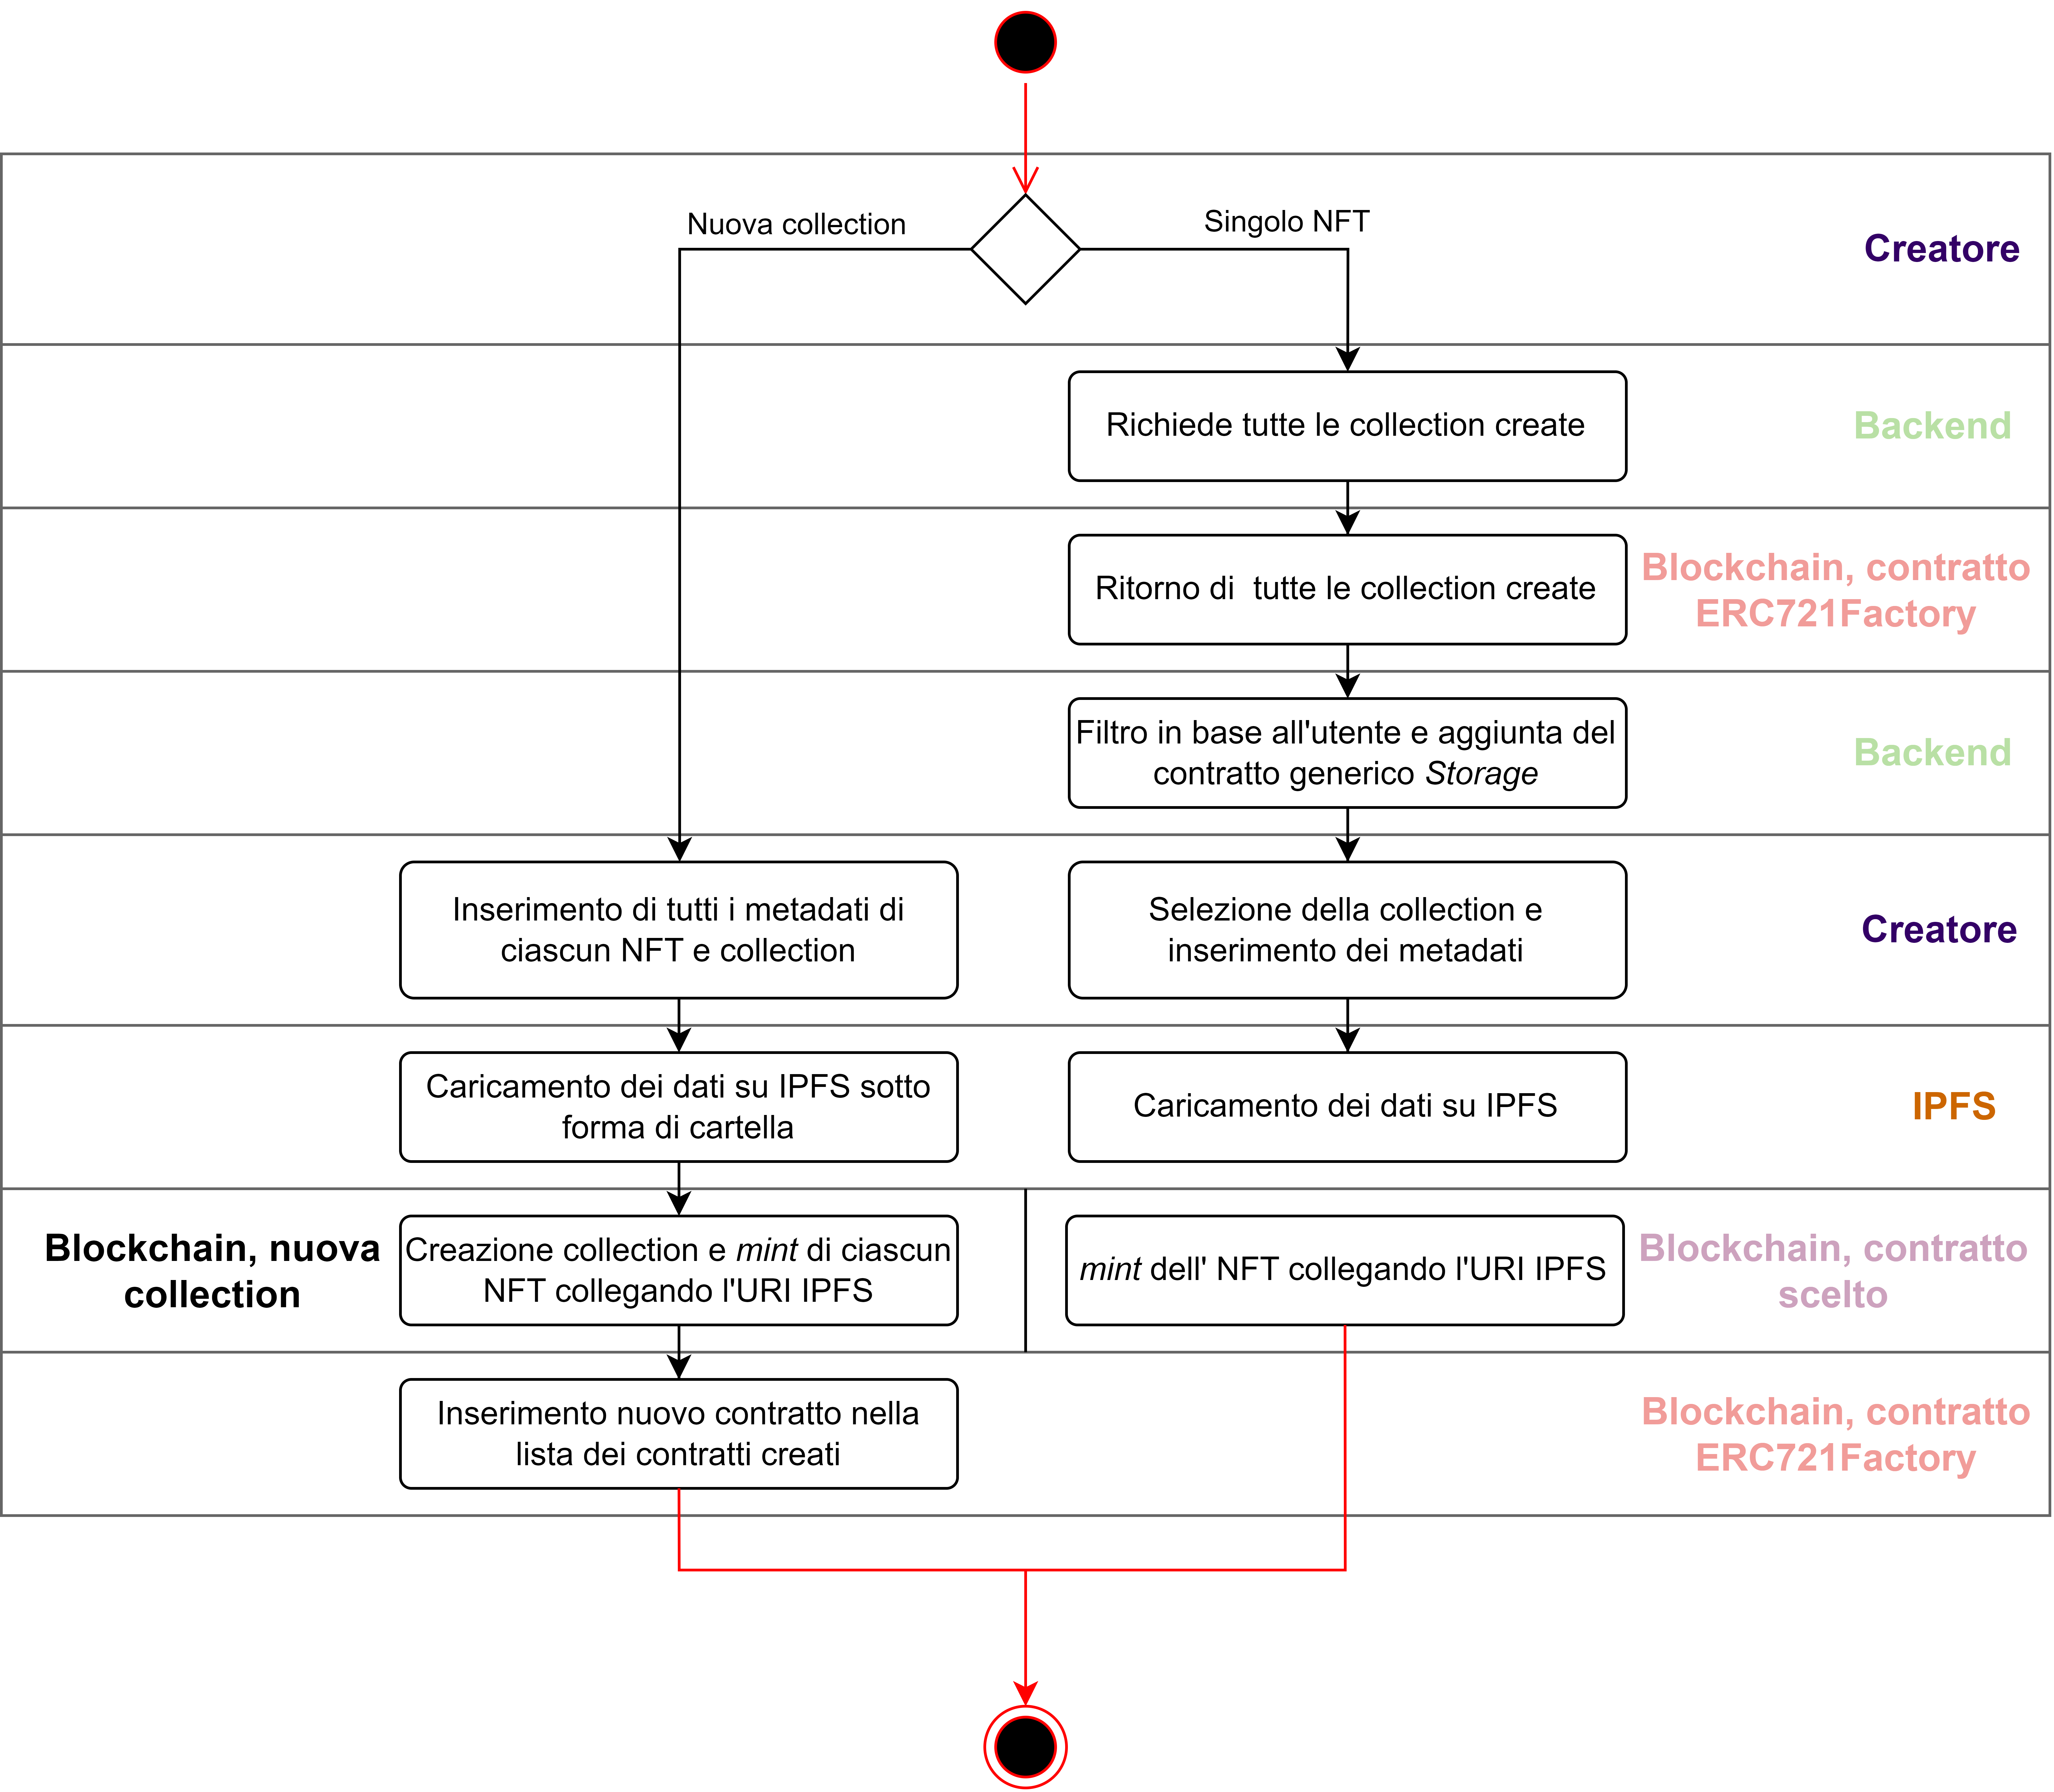
\includegraphics[width=1\textwidth]{images/creazioneNFT.png}
    \caption{Schema del processo di creazione di un NFT o più}
    \label{fig:creazioneNFT}
\end{figure}
